\documentclass[]{article}
\usepackage{multicol}
\usepackage{lmodern}
\usepackage{amssymb,amsmath}
\usepackage{ifxetex,ifluatex}
\usepackage{geometry}
\usepackage{listings}   % 代码支持
\usepackage{xcolor}     % 代码着色
\usepackage{multirow} % 表格支持
\usepackage{xeCJK} % 可以使用中文,而且有粗体,斜体
\usepackage{fixltx2e} % provides \textsubscript

\geometry{left=0cm,right=0cm,top=0cm,bottom=0cm}

\usepackage{graphicx,grffile}
\makeatletter
\def\maxwidth{\ifdim\Gin@nat@width>\linewidth\linewidth\else\Gin@nat@width\fi}
\def\maxheight{\ifdim\Gin@nat@height>\textheight\textheight\else\Gin@nat@height\fi}
\makeatother
% Scale images if necessary, so that they will not overflow the page
% margins by default, and it is still possible to overwrite the defaults
% using explicit options in \includegraphics[width, height, ...]{}
\setkeys{Gin}{width=\maxwidth,height=\maxheight,keepaspectratio}

\usepackage{parskip}

\setmonofont{Consolas}  % 等宽字体设定
\lstset{
        breaklines,
        % numbers=left, 
        % numberstyle=\tiny,keywordstyle=\color{blue!70},
        commentstyle=\color{red!50!green!50!blue!50},
        rulesepcolor=\color{red!20!green!20!blue!20},basicstyle=\linespread{1.0}\ttfamily\small,
        showstringspaces=false
}

% set default figure placement to htbp
\makeatletter
\def\fps@figure{htbp}
\makeatother

\date{}

% 添加水印
\usepackage{draftwatermark}
\usepackage{everypage}
\SetWatermarkText{Hosea@CC98}
\SetWatermarkLightness{0.9}
\SetWatermarkScale{0.7}
% 添加水印结束

\begin{document}
\begin{multicols}{3}

\paragraph{Created by Hosea@CC98}
\emph{半开卷\LaTeX}

\boxed{Code}
\begin{lstlisting}[language=c++]
bool Sphere::collision_handle(Vector3& pos) const {
    Scalar EPS = 0.05;
    Vector3 diff = pos - center;
    if (diff.norm() < radius + EPS) {
        // compare norm and radius
        diff.normalize(); // normalize vector diff
        diff *= radius + EPS;
        pos = center + diff;
        return true;
    }
    return false;
}
\end{lstlisting}

\boxed{Deadlock}

\textbf{死锁检测}如果 $T_i$ 等着 $T_j$ 解锁,那么等待图中就有 $T_i \to T_j$这条边。若等待图中有环,则存在死锁。
\textbf{死锁预防}\textit{predeclaration}:执行之前先检查会不会出现死锁,保证一个事务开始执行之前对涉及到的所
有的数据项都上锁。
\textit{graph-based protocol}:使用偏序来确定数据项上锁的顺序
\textit{wait-die}:被动。老的事务等待新事务释放,但是新的事务不等老的而是直接回滚。
\textit{wound-wait}:主动。老的事务强制让新的事务回滚而不等待其释放,新的事务会等老的事务结束。
\textit{Timeout-Based}:只等待一段时间,过了时间就回滚。容易实现,但是会导致starvation。
\textbf{死锁恢复}\textit{total rollback}:将事务abort之后重启;\textit{partial rollback}:不直接abort而实仅回滚到能解除死锁的状态。
\textbf{Multiple Granularity}允许数据项具有不同的大小,并定义数据粒度的层次结构,其中小粒度嵌套在大粒度中。可以用树形结构来表示。锁的粒度(level in tree where locking is done)\textit{fine granularity(lower in tree)高并发,高开销},\textit{coarse granularity(higher in tree) 低并发,低开销}。最高等级(根结点)是整个DB;最低等级(叶子结点)是区域,文件和记录。
\textbf{扩展的Lock Modes}
\textit{intention-shared (IS)}: indicates explicit locking at a lower level of the tree but only with shared locks.
\textit{intention-exclusive (IX)}: indicates explicit locking at a lower level with exclusive or shared locks.
\textit{shared and intention-exclusive (SIX)}: the subtree rooted by that node is locked explicitly in shared mode and explicit locking is being done at a lower level with exclusive-mode locks.
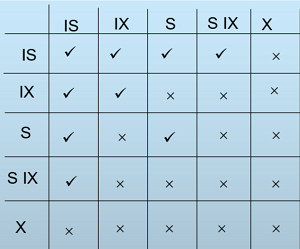
\includegraphics[height=20mm]{./img/lock.png}

\boxed{Triangle}
给定一个线段,随机取其中两点,将其分成三个线段,求这\textbf{三个线段能够首尾相接围成三角形的概率}。不妨设线段长度为$l$。记随机变量为$X,Y$分别表示分割点所在的坐标,则它们独立同分布于$U(0,l)$。不妨设$Y > X$(可以理解为只取$Y>X$的样本)。那么样本空间如图所示($l=4$)
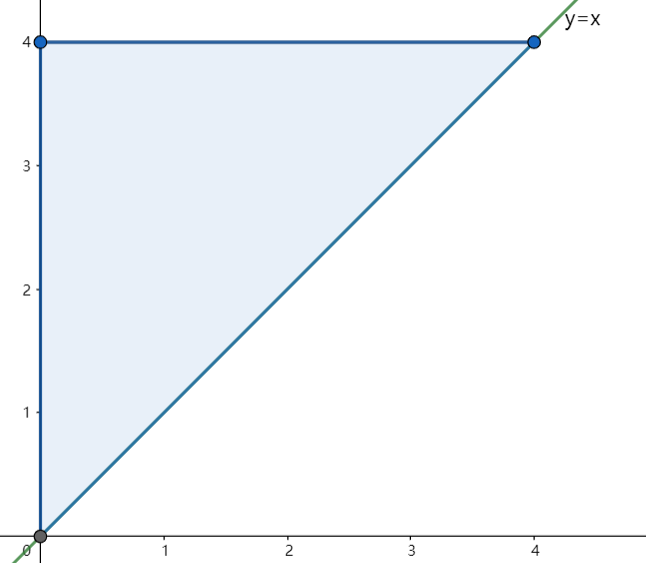
\includegraphics[height=10mm]{./img/1.png}
且三条线段的长度分别为$X,Y-X, l-Y$。这三条线段能围成三角形的充要条件是$X + (Y-X) > l -Y, X + (l - Y) > Y - X, (Y - X) + (l - Y) > X$。化简得$X < \frac{l}{2}, Y > \frac{l}{2}, Y < X + \frac{l}{2}$。可行域如图中绿色区域所示
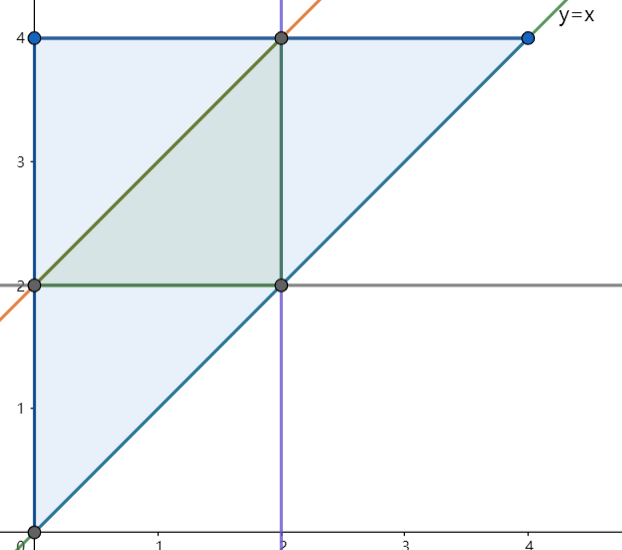
\includegraphics[height=10mm]{./img/2.png}
故\textbf{所求概率为$\frac{1}{4}$}。可行域内的每一个点$(x,y)$都意味着一种能围成三角形的分割方案$(x,y-x,l-y)$。

\boxed{Code}
\begin{lstlisting}[language=c++]
bool Sphere::collision_handle(Vector3& pos) const {
    Scalar EPS = 0.05;
    Vector3 diff = pos - center;
    if (diff.norm() < radius + EPS) {
        // compare norm and radius
        diff.normalize(); // normalize vector diff
        diff *= radius + EPS;
        pos = center + diff;
        return true;
    }
    return false;
}
\end{lstlisting}

\boxed{Deadlock}

\textbf{死锁检测}如果 $T_i$ 等着 $T_j$ 解锁,那么等待图中就有 $T_i \to T_j$这条边。若等待图中有环,则存在死锁。
\textbf{死锁预防}\textit{predeclaration}:执行之前先检查会不会出现死锁,保证一个事务开始执行之前对涉及到的所
有的数据项都上锁。
\textit{graph-based protocol}:使用偏序来确定数据项上锁的顺序
\textit{wait-die}:被动。老的事务等待新事务释放,但是新的事务不等老的而是直接回滚。
\textit{wound-wait}:主动。老的事务强制让新的事务回滚而不等待其释放,新的事务会等老的事务结束。
\textit{Timeout-Based}:只等待一段时间,过了时间就回滚。容易实现,但是会导致starvation。
\textbf{死锁恢复}\textit{total rollback}:将事务abort之后重启;\textit{partial rollback}:不直接abort而实仅回滚到能解除死锁的状态。
\textbf{Multiple Granularity}允许数据项具有不同的大小,并定义数据粒度的层次结构,其中小粒度嵌套在大粒度中。可以用树形结构来表示。锁的粒度(level in tree where locking is done)\textit{fine granularity(lower in tree)高并发,高开销},\textit{coarse granularity(higher in tree) 低并发,低开销}。最高等级(根结点)是整个DB;最低等级(叶子结点)是区域,文件和记录。
\textbf{扩展的Lock Modes}
\textit{intention-shared (IS)}: indicates explicit locking at a lower level of the tree but only with shared locks.
\textit{intention-exclusive (IX)}: indicates explicit locking at a lower level with exclusive or shared locks.
\textit{shared and intention-exclusive (SIX)}: the subtree rooted by that node is locked explicitly in shared mode and explicit locking is being done at a lower level with exclusive-mode locks.
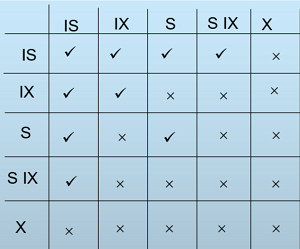
\includegraphics[height=20mm]{./img/lock.png}

\boxed{Triangle}
给定一个线段,随机取其中两点,将其分成三个线段,求这\textbf{三个线段能够首尾相接围成三角形的概率}。不妨设线段长度为$l$。记随机变量为$X,Y$分别表示分割点所在的坐标,则它们独立同分布于$U(0,l)$。不妨设$Y > X$(可以理解为只取$Y>X$的样本)。那么样本空间如图所示($l=4$)
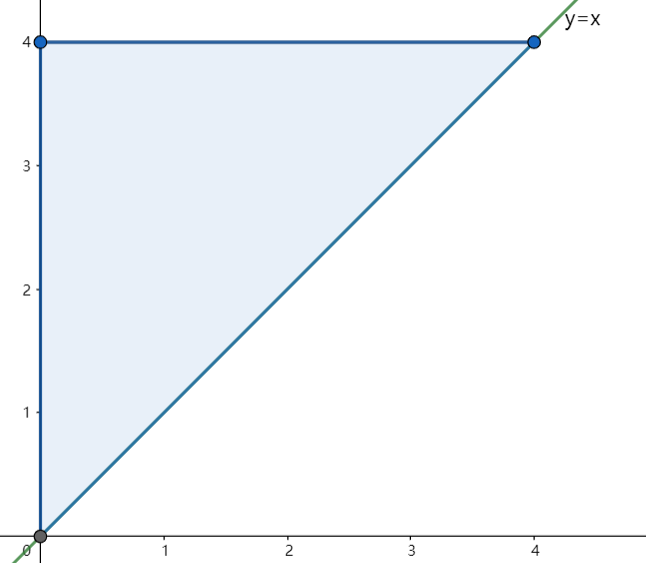
\includegraphics[height=10mm]{./img/1.png}
且三条线段的长度分别为$X,Y-X, l-Y$。这三条线段能围成三角形的充要条件是$X + (Y-X) > l -Y, X + (l - Y) > Y - X, (Y - X) + (l - Y) > X$。化简得$X < \frac{l}{2}, Y > \frac{l}{2}, Y < X + \frac{l}{2}$。可行域如图中绿色区域所示
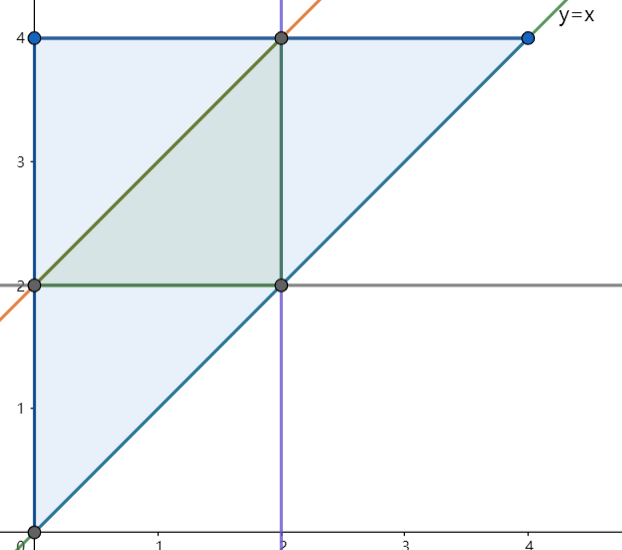
\includegraphics[height=10mm]{./img/2.png}
故\textbf{所求概率为$\frac{1}{4}$}。可行域内的每一个点$(x,y)$都意味着一种能围成三角形的分割方案$(x,y-x,l-y)$。

\boxed{Code}
\begin{lstlisting}[language=c++]
bool Sphere::collision_handle(Vector3& pos) const {
    Scalar EPS = 0.05;
    Vector3 diff = pos - center;
    if (diff.norm() < radius + EPS) {
        // compare norm and radius
        diff.normalize(); // normalize vector diff
        diff *= radius + EPS;
        pos = center + diff;
        return true;
    }
    return false;
}
\end{lstlisting}

\boxed{Deadlock}

\textbf{死锁检测}如果 $T_i$ 等着 $T_j$ 解锁,那么等待图中就有 $T_i \to T_j$这条边。若等待图中有环,则存在死锁。
\textbf{死锁预防}\textit{predeclaration}:执行之前先检查会不会出现死锁,保证一个事务开始执行之前对涉及到的所
有的数据项都上锁。
\textit{graph-based protocol}:使用偏序来确定数据项上锁的顺序
\textit{wait-die}:被动。老的事务等待新事务释放,但是新的事务不等老的而是直接回滚。
\textit{wound-wait}:主动。老的事务强制让新的事务回滚而不等待其释放,新的事务会等老的事务结束。
\textit{Timeout-Based}:只等待一段时间,过了时间就回滚。容易实现,但是会导致starvation。
\textbf{死锁恢复}\textit{total rollback}:将事务abort之后重启;\textit{partial rollback}:不直接abort而实仅回滚到能解除死锁的状态。
\textbf{Multiple Granularity}允许数据项具有不同的大小,并定义数据粒度的层次结构,其中小粒度嵌套在大粒度中。可以用树形结构来表示。锁的粒度(level in tree where locking is done)\textit{fine granularity(lower in tree)高并发,高开销},\textit{coarse granularity(higher in tree) 低并发,低开销}。最高等级(根结点)是整个DB;最低等级(叶子结点)是区域,文件和记录。
\textbf{扩展的Lock Modes}
\textit{intention-shared (IS)}: indicates explicit locking at a lower level of the tree but only with shared locks.
\textit{intention-exclusive (IX)}: indicates explicit locking at a lower level with exclusive or shared locks.
\textit{shared and intention-exclusive (SIX)}: the subtree rooted by that node is locked explicitly in shared mode and explicit locking is being done at a lower level with exclusive-mode locks.
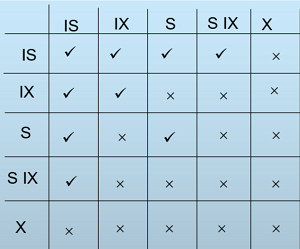
\includegraphics[height=20mm]{./img/lock.png}

\boxed{Triangle}
给定一个线段,随机取其中两点,将其分成三个线段,求这\textbf{三个线段能够首尾相接围成三角形的概率}。不妨设线段长度为$l$。记随机变量为$X,Y$分别表示分割点所在的坐标,则它们独立同分布于$U(0,l)$。不妨设$Y > X$(可以理解为只取$Y>X$的样本)。那么样本空间如图所示($l=4$)
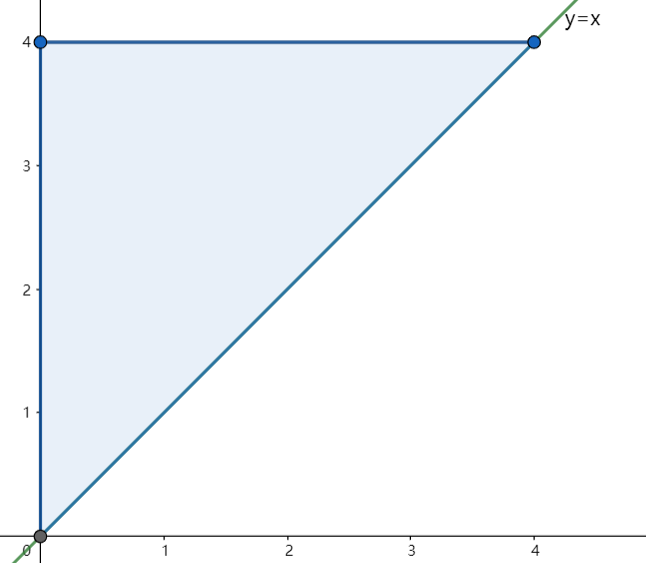
\includegraphics[height=10mm]{./img/1.png}
且三条线段的长度分别为$X,Y-X, l-Y$。这三条线段能围成三角形的充要条件是$X + (Y-X) > l -Y, X + (l - Y) > Y - X, (Y - X) + (l - Y) > X$。化简得$X < \frac{l}{2}, Y > \frac{l}{2}, Y < X + \frac{l}{2}$。可行域如图中绿色区域所示
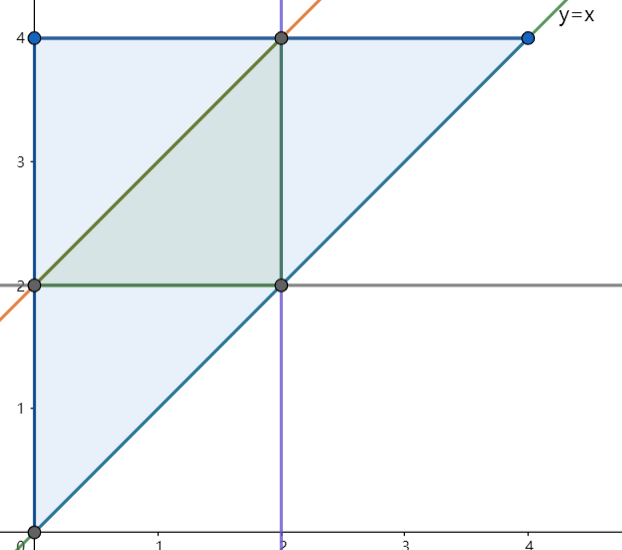
\includegraphics[height=10mm]{./img/2.png}
故\textbf{所求概率为$\frac{1}{4}$}。可行域内的每一个点$(x,y)$都意味着一种能围成三角形的分割方案$(x,y-x,l-y)$。

\boxed{Code}
\begin{lstlisting}[language=c++]
bool Sphere::collision_handle(Vector3& pos) const {
    Scalar EPS = 0.05;
    Vector3 diff = pos - center;
    if (diff.norm() < radius + EPS) {
        // compare norm and radius
        diff.normalize(); // normalize vector diff
        diff *= radius + EPS;
        pos = center + diff;
        return true;
    }
    return false;
}
\end{lstlisting}

\boxed{Deadlock}

\textbf{死锁检测}如果 $T_i$ 等着 $T_j$ 解锁,那么等待图中就有 $T_i \to T_j$这条边。若等待图中有环,则存在死锁。
\textbf{死锁预防}\textit{predeclaration}:执行之前先检查会不会出现死锁,保证一个事务开始执行之前对涉及到的所
有的数据项都上锁。
\textit{graph-based protocol}:使用偏序来确定数据项上锁的顺序
\textit{wait-die}:被动。老的事务等待新事务释放,但是新的事务不等老的而是直接回滚。
\textit{wound-wait}:主动。老的事务强制让新的事务回滚而不等待其释放,新的事务会等老的事务结束。
\textit{Timeout-Based}:只等待一段时间,过了时间就回滚。容易实现,但是会导致starvation。
\textbf{死锁恢复}\textit{total rollback}:将事务abort之后重启;\textit{partial rollback}:不直接abort而实仅回滚到能解除死锁的状态。
\textbf{Multiple Granularity}允许数据项具有不同的大小,并定义数据粒度的层次结构,其中小粒度嵌套在大粒度中。可以用树形结构来表示。锁的粒度(level in tree where locking is done)\textit{fine granularity(lower in tree)高并发,高开销},\textit{coarse granularity(higher in tree) 低并发,低开销}。最高等级(根结点)是整个DB;最低等级(叶子结点)是区域,文件和记录。
\textbf{扩展的Lock Modes}
\textit{intention-shared (IS)}: indicates explicit locking at a lower level of the tree but only with shared locks.
\textit{intention-exclusive (IX)}: indicates explicit locking at a lower level with exclusive or shared locks.
\textit{shared and intention-exclusive (SIX)}: the subtree rooted by that node is locked explicitly in shared mode and explicit locking is being done at a lower level with exclusive-mode locks.
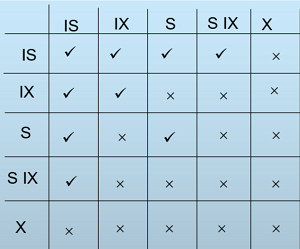
\includegraphics[height=20mm]{./img/lock.png}

\boxed{Triangle}
给定一个线段,随机取其中两点,将其分成三个线段,求这\textbf{三个线段能够首尾相接围成三角形的概率}。不妨设线段长度为$l$。记随机变量为$X,Y$分别表示分割点所在的坐标,则它们独立同分布于$U(0,l)$。不妨设$Y > X$(可以理解为只取$Y>X$的样本)。那么样本空间如图所示($l=4$)
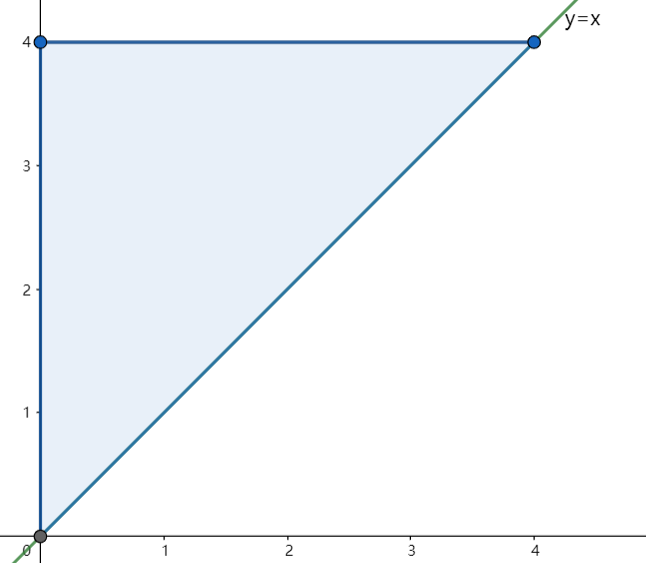
\includegraphics[height=10mm]{./img/1.png}
且三条线段的长度分别为$X,Y-X, l-Y$。这三条线段能围成三角形的充要条件是$X + (Y-X) > l -Y, X + (l - Y) > Y - X, (Y - X) + (l - Y) > X$。化简得$X < \frac{l}{2}, Y > \frac{l}{2}, Y < X + \frac{l}{2}$。可行域如图中绿色区域所示
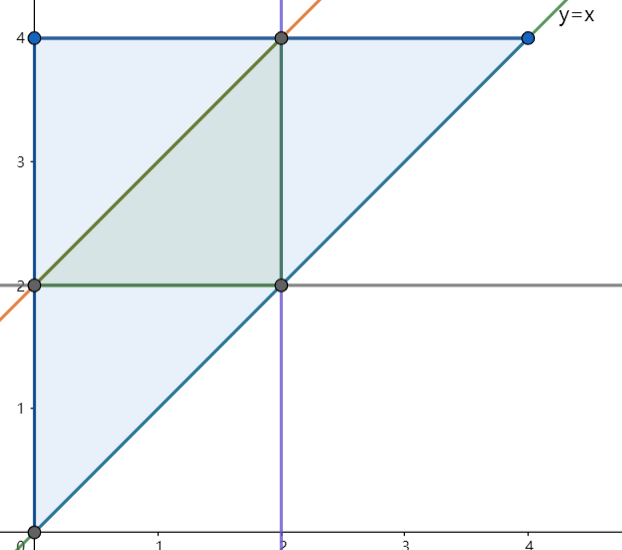
\includegraphics[height=10mm]{./img/2.png}
故\textbf{所求概率为$\frac{1}{4}$}。可行域内的每一个点$(x,y)$都意味着一种能围成三角形的分割方案$(x,y-x,l-y)$。

\boxed{Code}
\begin{lstlisting}[language=c++]
bool Sphere::collision_handle(Vector3& pos) const {
    Scalar EPS = 0.05;
    Vector3 diff = pos - center;
    if (diff.norm() < radius + EPS) {
        // compare norm and radius
        diff.normalize(); // normalize vector diff
        diff *= radius + EPS;
        pos = center + diff;
        return true;
    }
    return false;
}
\end{lstlisting}

\boxed{Deadlock}

\textbf{死锁检测}如果 $T_i$ 等着 $T_j$ 解锁,那么等待图中就有 $T_i \to T_j$这条边。若等待图中有环,则存在死锁。
\textbf{死锁预防}\textit{predeclaration}:执行之前先检查会不会出现死锁,保证一个事务开始执行之前对涉及到的所
有的数据项都上锁。
\textit{graph-based protocol}:使用偏序来确定数据项上锁的顺序
\textit{wait-die}:被动。老的事务等待新事务释放,但是新的事务不等老的而是直接回滚。
\textit{wound-wait}:主动。老的事务强制让新的事务回滚而不等待其释放,新的事务会等老的事务结束。
\textit{Timeout-Based}:只等待一段时间,过了时间就回滚。容易实现,但是会导致starvation。
\textbf{死锁恢复}\textit{total rollback}:将事务abort之后重启;\textit{partial rollback}:不直接abort而实仅回滚到能解除死锁的状态。
\textbf{Multiple Granularity}允许数据项具有不同的大小,并定义数据粒度的层次结构,其中小粒度嵌套在大粒度中。可以用树形结构来表示。锁的粒度(level in tree where locking is done)\textit{fine granularity(lower in tree)高并发,高开销},\textit{coarse granularity(higher in tree) 低并发,低开销}。最高等级(根结点)是整个DB;最低等级(叶子结点)是区域,文件和记录。
\textbf{扩展的Lock Modes}
\textit{intention-shared (IS)}: indicates explicit locking at a lower level of the tree but only with shared locks.
\textit{intention-exclusive (IX)}: indicates explicit locking at a lower level with exclusive or shared locks.
\textit{shared and intention-exclusive (SIX)}: the subtree rooted by that node is locked explicitly in shared mode and explicit locking is being done at a lower level with exclusive-mode locks.
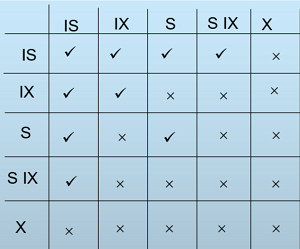
\includegraphics[height=20mm]{./img/lock.png}

\boxed{Triangle}
给定一个线段,随机取其中两点,将其分成三个线段,求这\textbf{三个线段能够首尾相接围成三角形的概率}。不妨设线段长度为$l$。记随机变量为$X,Y$分别表示分割点所在的坐标,则它们独立同分布于$U(0,l)$。不妨设$Y > X$(可以理解为只取$Y>X$的样本)。那么样本空间如图所示($l=4$)
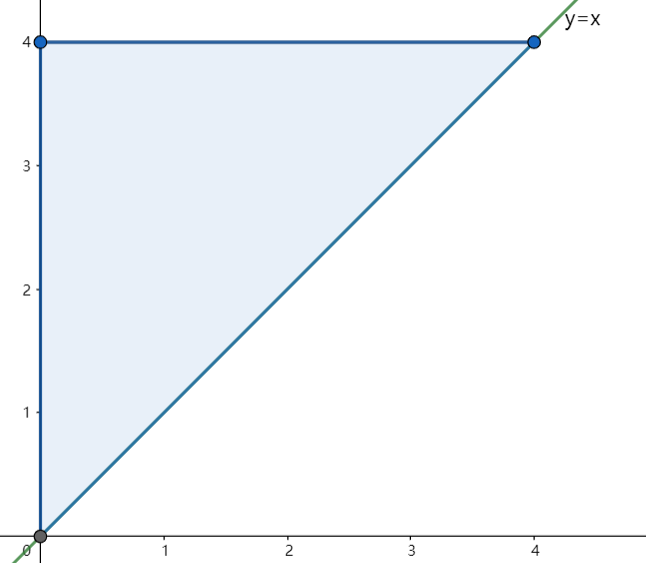
\includegraphics[height=10mm]{./img/1.png}
且三条线段的长度分别为$X,Y-X, l-Y$。这三条线段能围成三角形的充要条件是$X + (Y-X) > l -Y, X + (l - Y) > Y - X, (Y - X) + (l - Y) > X$。化简得$X < \frac{l}{2}, Y > \frac{l}{2}, Y < X + \frac{l}{2}$。可行域如图中绿色区域所示
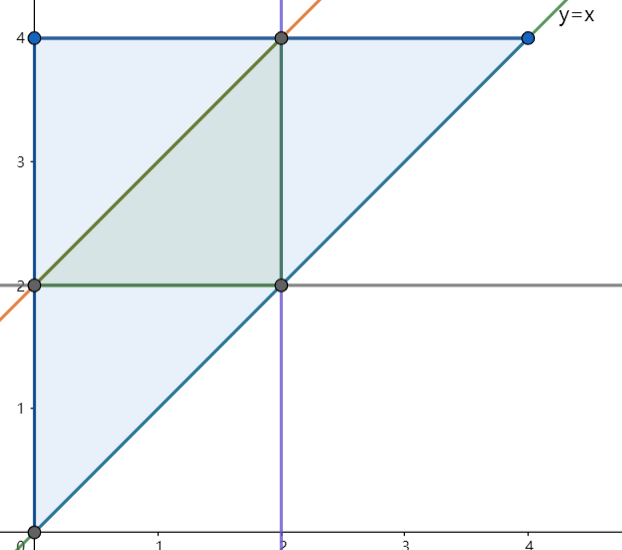
\includegraphics[height=10mm]{./img/2.png}
故\textbf{所求概率为$\frac{1}{4}$}。可行域内的每一个点$(x,y)$都意味着一种能围成三角形的分割方案$(x,y-x,l-y)$。

\boxed{Code}
\begin{lstlisting}[language=c++]
bool Sphere::collision_handle(Vector3& pos) const {
    Scalar EPS = 0.05;
    Vector3 diff = pos - center;
    if (diff.norm() < radius + EPS) {
        // compare norm and radius
        diff.normalize(); // normalize vector diff
        diff *= radius + EPS;
        pos = center + diff;
        return true;
    }
    return false;
}
bool Sphere::collision_handle(Vector3& pos) const {
    Scalar EPS = 0.05;
    Vector3 diff = pos - center;
    if (diff.norm() < radius + EPS) {
        // compare norm and radius
        diff.normalize(); // normalize vector diff
        diff *= radius + EPS;
        pos = center + diff;
        return true;
    }
    return false;
}
\end{lstlisting}





\end{multicols}
\end{document}
